\documentclass{elsarticle}
\usepackage{amssymb}
\usepackage{amsmath}
\usepackage{bigdelim}
\usepackage{multirow}
\usepackage{hyperref}
\usepackage{graphics}
\usepackage{algorithm}
\usepackage{algorithmic}

%\usepackage{algorithmicx}
\journal{Expert System with Applications}

\newtheorem{definition}{Definition}


\begin{document}

\begin{frontmatter}
\title{A Complex Network Model of Knowledge Collaboration in Virtual Community: Based on Wiki Community
}
\author[buaa]{Jun Wang}
\ead{king.wang@buaa.edu.cn}

\author[buaa]{Yunpeng Wu}
\ead{yunpeng.wu@sem.buaa.edu.cn}

\author[buaa]{Xin Jin}
\ead{sssss}

\address[buaa]{School of Economics and Management, Beihang University, 
Beijing 100083, P.R. China}

\begin{abstract}
  
\end{abstract}

\begin{keyword}
Wikipedia, Knowledge collaboration network, Scale-free structure,
Small-world effect, Topic Approximation, scale ratio
  
\end{keyword}
\end{frontmatter}

\section{Introduction}
\label{sec:introduction}

In the past few years, complex network is being infiltrated into sociology, mathematics, life sciences, engineering and many other different areas, the scientific understanding to the quantitative and qualitative characteristics of complex network has become a challenging and important issues of scientific research in the Internet era, and even referred to as "the network's new science"[1-2]. Social networks, which are an important examples of complex networks, have many similar properties with complex networks [3]. For example, the short length of the average shortest-path distance, the high value of the clustering coefficient and the scale-free distribution of connectivity are some of the common properties of those networks [4-6].In other words, there are many similar conclusions among them, such as “small worlds” effect[7],scale-free[8], power law[9] and so on. 

In recent years, bipartite networks have attracted more and more people's attention [10-13]. Factuallyt, many real-world networks are naturally bipartite, such as the actors-films network [11], the Scientist Co-authorship Collaboration network [12-13], the knowledge-cooperation network and so on.

Wiki system as the typical knowledge-cooperation newtork and virtual practice community has become more and more popular in knowledge management system field. It is an important approach to publish on-line information and a different way to collaborate. They can be characterized as ‘‘ultra-lightweight’’ content management systems [14]. Wiki is a method for knowledge cooperation and refers to a collaborative hyper medium that allows for continuous communication within a research team and the constant evolution of content [15].Wikis are used for a diversified number of applications: some as databases for research and writing, as personal information manager, as collaborative tool between teams to create and maintain documents that need to be updated frequently, etc.

Wiki network is different from other social networks on the WWW,such as Sina Blog. The collaboration in Blog is non-themed or variable- themed. However, for the same theme, the collaboration in wiki is expanding denotedly and connotedly. It will talk about a topic with a very full depth [16].

In the current studies, complex network has shown a lot of valuable properties [7-13,17]. This paper focuses on two aspects: the wiki one-dimensional network, ties connected between users; the bipartite network, the ties connected users and topics. Through an empirical study of en-Wikipedia network’s data which is from January 2004 to January 2008, we discover that many properties of wiki network are similar with other networks. 

The rest of the paper is organized as follows. In section II, we
introduce the complex social network mould wiki-based knowledge
collaboration. The empirical analysis of the one-dimensional
properties is presented in section III. On the meanwhile, section IV
proposes the pilot study of the wiki bipartite network, namely, the
relationship between network properties and scale. Section V is
devoted to our conclusions and discussions.

\section{The network structure of Wiki-based knowledge collaboration}
\label{sec:netw-struct-wiki}

Wikipedia is a typical Knowledge collaboration- oriented virtual community, in which the group who has the same interest in the same topic can communicate and interact with each other through topic pages to participate in the knowledge collaboration activities. Wikipedia can be depicted as an open content encyclopedia,the open materials of which allow unrestricted access to any third party to copy, modify, thus, it  provides great convenience for people from various sectors. On the meantime, the users can increase their knowledge and enrich themselves. As of April 25, 2009, according to Wikipedia statistics (Wiki Stats Statistics) [18], the English version has 16,550,111 entries, user groups have been 9,505,160.Over a period of time, there will be a certain number of user groups to participate in the discussion of a topic.

As to the characteristics of Wikipedia knowledge collaboration network, the authors of this paper build a collaborative Wiki-based knowledge network model, as shown in Figure 1. There are also two types of ties: C and A: C is the collaboration among users, shown as white lines in Fig.1, while the A express the affiliation between T and U, shown as dark color lines in Fig.1. The collaboration relationship among C ties comes into being through participating in the A ties discussions.  

\begin{figure}[h]
  \centering
  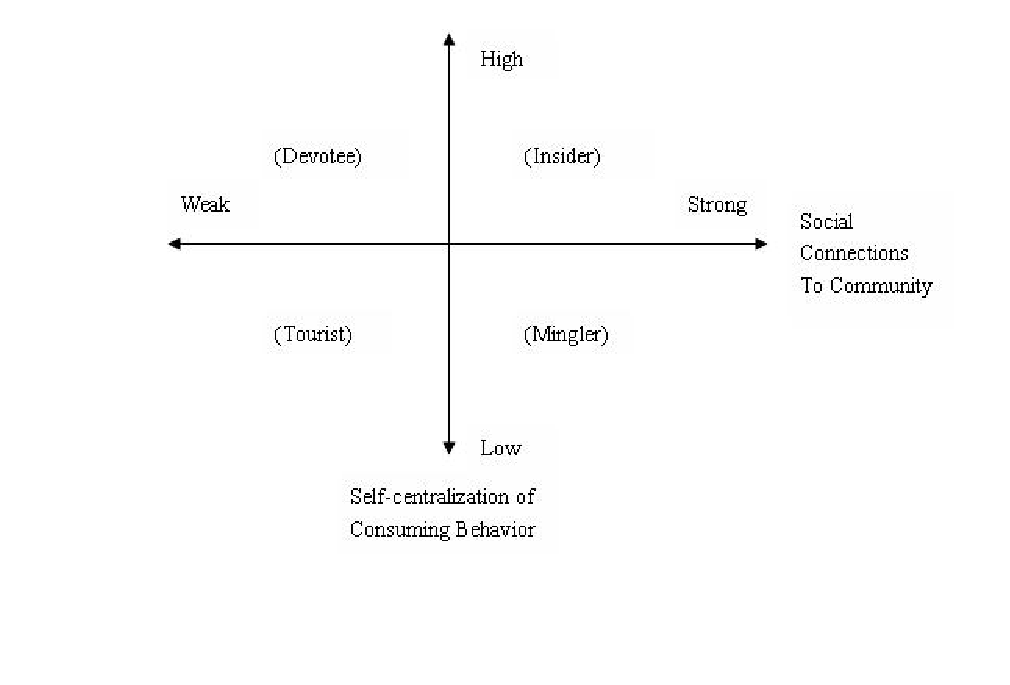
\includegraphics{01}
  \caption{The Two-dimensional, Wiki-based Knowledge Collaboration Network Mould}
\end{figure}

From the network model in figure 1, it is easily found that this model
includes two complex networks: one-dimensional networks of
single-layer and bipartite two-dimensional networks. 

In the single-layer networks, all the users in the same Topic collaboration process builds Undirected and Unweighted Complete Sub-graph (UUCSG), shown as [u1-u2] [u3-u6] [u6-u10] [u9-u12] in Fig.1.The entire single-layer network is composed of n UUCSGs, in which N represents the number of Topics. The whole network can be expressed as an adjacency matrix “Bu”.

 the bipartite networks, the UUCSG is constructed by all the UUCSGs in
 the single-layer networks and the topics which the UUCSG belong
 to. The number of nodes is equal to the numbers of the User
 nodes. Therefore, the bipartite networks can be described as an
 adjacency matrix “Bt”. The ratio between Users and Topics exists in
 the bipartite networks, which is called scale ratio and can be
 described as
 \begin{math}
 W = N_{user}/N_{topic}   
 \end{math}
This model does not clearly define the direction of the relationship, thus, the model belongs to Undirected and Unweighted Complete Sub-graph. However, such network model vividly displays virtual communities of practice networks which aims for knowledge collaboration and innovation, such as Wikipedia.



\begin{align*}
  \begin{matrix} 
 &u_1 & u_2 \\  
 u_1\ldelim[{2}{0.1cm}&1&0&\rdelim]{2}{0.1cm}\\
 u_2 &0&1\\
\end{matrix}
& \qquad \qquad 
\begin{matrix}  & T_1 & T_2 \\ 
 u_1\ldelim[{2}{0.1cm}&1&0&\rdelim]{2}{0.1cm}\\
 u_2&1&0 \\
\end{matrix}
\end{align*}

\section{The empirical study of single-dimensional Wiki-based knowledge collaboration network}
\label{sec:empir-study-single}

Since Wikipedia provides all kinds of comprehensive, convenient, and accurate archives of history data which are stored in the form of . XML and SQL files, the researchers can download for free according to their different requirements. We choose “enwiki-20081008-stub-meta-history.xml”[19] as our research data. These files contain no page text, only revision metadata before December 8th 2008. Because the Wikipedia community was in an unstable phase before 2003, we choose the data from 2004 to 2008. In order to better observe the changes of the network properties at different time periods, we divided the time duration into months, build 48 sub-networks of each month from January 2004 to December 2007 and calculate the special data of the 48 sub-networks.

The data on access in this study are filtered and cleared in the following steps. Step 1, screen out all contributors data in the above-mentioned time periods and all the related contributors versions, topic pages data. Then clear the data twice. Step 2: do the first clearing: exclude the data which have no user ids but only IP addresses, since we are unable to check the identity and track his activities without user ID. Factually, we need to track the contributors’ activities and user id is the identification to be followed up. Step 3: do the second clearing: delete isolated nodes, namely, those nodes which have only one user under a topic. In this study, it is admitted that there is no collaboration relationship between this user and other users under such topic.

In order to illustrate the data changes, ultimately the 24 odd-numbered subnets are selected as representatives to describe the network characteristics. The summary of the cleared network data are shown in table 1, which clearly describes the static parameters changes of Wiki-based knowledge collaboration networks over time. The increase of Wiki-based knowledge collaboration networks is decided by the growth of the Wikipedia practice community. With the Wikipedia culture is receiving increasing attention since 2004, the scale of the Wikipedia virtual community is gradually expanding. And there were more than 1400 million pages in Wikipedia until October 2008. However, it is also obvious that the network scale grew quickly from 2004 to the mid of 2007, but declined later.
% Table generated by Excel2LaTeX from sheet 'Working'
\begin{table}[htbp]
 
  \caption{Add caption}
   \begin{tabular}{lllllll}
        & Users & Pages & W &  \parbox{1.4
cm}{Average Degree} &  \parbox{1.7cm}{Clustering Coefficient} &  Density \\\hline
      {\bf Jan-04} & 2634  & 18650 & 0.141233 & 83.125 & 0.642991 & 0.063141 \\
    {\bf Mar-04} & 4807  & 37733 & 0.127395 & 85.467 & 0.640963 & 0.035567 \\
    {\bf May-04} & 5344  & 35688 & 0.149742 & 88.263 & 0.629839 & 0.033039 \\
    {\bf Jul-04} & 6814  & 57986 & 0.117511 & 94.662 & 0.651261 & 0.027789 \\
    {\bf Sep-04} & 8621  & 66186 & 0.130254 & 113.226 & 0.648146 & 0.026271 \\
    {\bf Nov-04} & 11757 & 97336 & 0.120788 & 116.668 & 0.654176 & 0.019848 \\
    {\bf Jan-05} & 12343 & 61389 & 0.201062 & 91.989 & 0.632225 & 0.014907 \\
    {\bf Mar-05} & 15943 & 91034 & 0.175132 & 102.796 & 0.630041 & 0.012896 \\
    {\bf May-05} & 20323 & 113260 & 0.179437 & 104.417 & 0.678814 & 0.010276 \\
    {\bf Jul-05} & 27127 & 140591 & 0.19295 & 135.279 & 0.647197 & 0.009974 \\
    {\bf Sep-05} & 30125 & 153697 & 0.196003 & 125.932 & 0.650241 & 0.008361 \\
    {\bf Nov-05} & 37182 & 190484 & 0.195197 & 117.661 & 0.662213 & 0.006329 \\
    {\bf Jan-06} & 61349 & 276782 & 0.221651 & 156.882 & 0.676517 & 0.005114 \\
    {\bf Mar-06} & 83577 & 331995 & 0.251742 & 157.1 & 0.7016 & 0.003759 \\
    {\bf May-06} & 95454 & 336581 & 0.283599 & 157.751 & 0.705743 & 0.003305 \\
    {\bf Jul-06} & 104253 & 371719 & 0.280462 & 152.648 & 0.712564 & 0.002928 \\
    {\bf Sep-06} & 122794 & 395049 & 0.310832 & 151.984 & 0.697645 & 0.002475 \\
    {\bf Nov-06} & 138858 & 396855 & 0.349896 & 154.183 & 0.724345 & 0.002221 \\
    {\bf Jan-07} & 154494 & 449403 & 0.343776 & 151.459 & 0.720432 & 0.001961 \\
    {\bf Mar-07} & 168900 & 492561 & 0.342902 & 176.884 & 0.719482 & 0.002095 \\
    {\bf May-07} & 160008 & 474705 & 0.337068 & 224.048 & 0.693921 & 0.0028 \\
    {\bf Jul-07} & 138543 & 432391 & 0.320411 & 174.423 & 0.701221 & 0.002518 \\
    {\bf Sep-07} & 146961 & 454726 & 0.323186 & 230.81 & 0.702132 & 0.003141 \\
    {\bf Nov-07} & 145782 & 440376 & 0.33104 & 189.126 & 0.71322 & 0.002595 \\
       \end{tabular}
  \label{tab:addlabel}
\end{table}
In order to observe the network changes with time in more details, this paper gives a more figurative description of the topological properties of the one-dimensional complex network of knowledge-oriented collaboration. And the description expands from five aspects: power Law, average degree, clustering coefficient, small world and hierarchical network.

\subsection{The analysis of scale-free structure}
\label{sec:analysis-scale-free}

In network description, degree distribution attracts more and more researchers’ attention because of its inherent important topology information and network evolution information. In order to explain the generation mechanism of power-law distribution, Barabási and Albert proposed a scale-free network model, known as the BA model now[20].  The degree of the node refers to the number of the node's adjacent nodes or the number of adjacent edges. In Wiki-based knowledge collaboration network descriptions, the degree of Node i is described as in (1): 
\begin{equation}
  K_i=\sum_{j\in\mu_i}C_{ij}
\end{equation}

$\mu_j$represents the adjacency matrix of the user node. If nodes $i$
and $j$ are linked, the value  is 1, otherwise 0. Degree distribution
refers to the probability of a node with exact degree $k$ in the
selected network. Studies show that degree distribution of BA
scale-free network is in line with the shifted power-law, that is
$P(k)\thicksim k^\gamma+\alpha$  , and the $\gamma$ and $\alpha$ are both
constants. 

上述24个Wikipedia子网的度分布$P(k)$ 在双对数坐标下的曲线,如图2所示。
The degree distributions of the above 24 Wikipedia subnet are
displayed as curves in double logarithmic coordinates, as shown in
Figure 2. To show conveniently, each subgraph in Figure 2 identifies
the subnets of three months.

Master equation method is adopted to further analyze degree
distributions of the above collaboration networks[21]. Degree
distribution function of the BA network can be similarly described by
the Power-law function with Power index for the 3. As Figure 2 shows,
the slope of the power-law distribution function of the Wiki-based
collaborative knowledge network in log-log coordinates is approximate
to (1E-2-1E-3), and has similar values like m (the intercept of Fit
Linear is approximate). Wiki-based知识协同网络的幂律分布函数在双对数坐
标下,斜率近似为(1E-2—1E-3),并且具有相近似的m值(Fit Linear的截距近
似)。Therefore, wiki-based knowledge collaboration network is a type
of BA scale-free network, and its characteristics which conform to the
BA scale-free network are:

Growth: The size of BA network is continually growing. Every day there
are many new users joining in the wiki-based knowledge collaboration
community. According to the internal data of
Wikipedia(http://stats.wikimedia.org/EN/TablesWikipediansNew.htm),
there are a certain amount of new wikipedians participating in the
collaborative activities every day. 

Preferential Attachment: The new node prefers to connect with those
“big nodes” with higher degree. This phenomenon is also known as "the
rich get richer" or "Matthew Effect". In wiki-based knowledge
collaboration network, new wikipedians tend to participate in editing
the pages whose editors are “big nodes”. The way of network evolution
is moving closer to the central node, thereby forms the polarization
between the rich and the poor. The Scale-free networks can grow from
very few nodes to a complex network with a large number of nodes. Here
the so-called “big” nodes are referred to as “active users.” When the
quantity of the network nodes grows to a certain scale, the network
will indicate that: only a few users have a large number of connected
nodes, while a great many users only have a small number of
connections, namely, which demonstrates the “long tail” phenomenon. 

\begin{figure}[htpb]
  \centering
  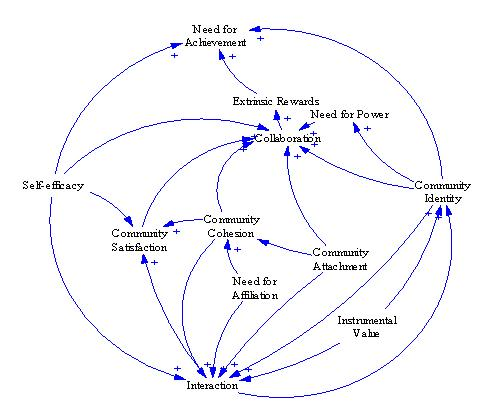
\includegraphics{03}
  \caption{The Changes curve of the average degree over time}
\end{figure}

\subsection{The changes of average degree}
\label{sec:chang-aver-degr}

With the development of the Wiki culture, such knowledge collaboration
and innovation pattern is attaching more and more attentions. On the
meantime, the number of the Wiki users is increasing, as Figure
1shows. There are two reasons for the increase of the users: the first
is the increasing new topics. According to the internal data of
Wikipedia, new entries of wiki network have increased each year [22],
thus, attracts more users to join in the topics of common concern. The
second is that more and more users are participating in the
contribution under the existing topics. Therefore, the average degree
is introduced to describe the number of relationship within Wiki
network, namely,$AverageDegree = \sum_iK_i/\text{Number of Users}$

The change curve of average degree over time is shown in Figure 3. Obviously, the average degree presents a certain cyclical change over time, and there is an upward shocks trend, which indicates the number of the “innate relations” of the knowledge collaborative networks shows cyclical fluctuations and more closely linked trend. In the Wikipedia community, average degree concussion is caused by the shock of the Topic node. Take the topic “the Festival” as example, the number of the editing increases apparently in January and February of each year. Another example is "financial crisis", and the dynamism of it increases sharply in 2008. Therefore, the average degree will be showing a shock for a long time, which is closely related to the degree of concern within Wikipedia topic.

\subsection{ The changes of Clustering Coefficient}
\label{sec:chang-clust-coeff}

Clustering Coefficient, also known as Congregate Extent, describes the
clustering effect of the complex network, while reflects the property
of “Like attract like”. Suppose that the degree of a node $i$ in the
network is $k_i$  , $k_i$  -nodes which are connected with $i$ are
known as Node i’s neighbors. Then $C_i$ which refers to the Clustering
Coefficient of the Node $i$ can be defined as the ratio between the
real number of the edges among the $k_i$  nodes and the possible total
number of edges $k_i(k_i-1)/2$ : $C_i=2E_i/k_i(k_i-1)$ . And the
Clustering Coefficient of the whole network C is the average of all
the nodes’ clustering coefficient.

The changes of the Clustering Coefficient of the knowledge
collaboration one-dimensional network are shown in Figure 4. In
one-dimensional network, C value will tend to a certain non-zero
constant with the increasing of network size, that is, when
$N\rightarrow\infty,C=O(1)$ . The Clustering Coefficient of the
free-scale network BA can be defined as $C=\beta[\ln(t)]^2/t$ , and
is network evolution constant.

In wiki-based knowledge collaboration networks, the Clustering Coefficients in period 2004 to 2008 are presented in Fig.3. The result shows that the Clustering Coefficient averages to 0.55. In fact, many types of complex networks, especially social networks, aren’t entirely random network. In a way, they show the "people to group" features. This conclusion is obvious, according to the definition of communities of practice: the people who pay attention to certain subject, and with strong passion for this topic, increase their knowledge and skills through communicating and exchanging knowledge in this field with each other sustained[18]. As a typical virtual community of practice, the members participate in editing the pages of some topics  in accordance with their interests, hobbies, professional. In general, wikipedians show the "people to group" features.

Wiki-based知识协同网络的集聚程度随时间的变化如图4所示(上一段已经提过),In wiki-based knowledge collaboration networks, the Clustering Coefficients changes are presented in Fig.4. The results of the experiments show that the Clustering Coefficient focus on about 0.55. Threrefore, it is natural to draw the conclusion that many types of complex networks, especially social networks, aren’t entirely random networks, on the contrary, they have the characteristic of “Like attracts like.” Practice community is defined as: the people who pay close attention to a certain subject and hold strong passion for this topic, furthermore, they increase their knowledge and skills in this field through sustained communicating and exchanging knowledge with each other [24]. As a typical virtual community of practice, the members in wikipedia community participate in editing the pages of some topics in accordance with their interests, hobbies and professions, naturally, there exists a feature of “People groups” among them.
\begin{figure}[htpb]
  \centering
  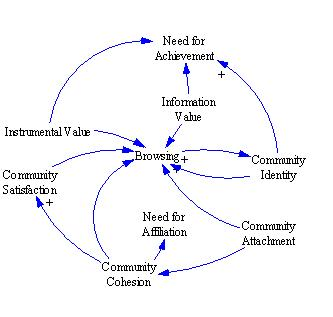
\includegraphics{04}
  \caption{ The Clustering Coefficient Changes with Time}
\end{figure}

\subsection{“Small world” phenomenon }
\label{sec:small-world-phen}

Small world phenomenon reflects a kind of social network characteristics, that is, most of the people and their friends are in the same circle of people. On the other hand, there are some people living far away, or even living in a foreign country. Many studies have shown that small-world phenomenon exists in many real networks. This network has two characteristics: shorter average path length and higher clustering coefficient. Here, average path length L means the minimum number of edges connecting a pair of vertices, averaged over all pairs of vertices, which plays an important role in both transportation and communication within a network. Because of the large calculation scale of the average path and the limitation of calculation, this study only calculates and analyzes the average distances of the 6 sub-networks of the 1st, 18th, and 35th weeks of 2004 and 2005 whose size are still relatively small, as shown in table 2.

The results of table 2 indicate two conclusions. On the one hand, the clustering coefficients are around 0.5, which is higher. On the other hand, the average path length is small (<4), that is, any two people in the network can find each other through less than 4 individuals on average. Therefore, wiki-based knowledge collaboration networks turn on apparent property of small-world phonamenon. 因此,在知识协同网络中表现出明显的小世界现象。

\begin{table}[htpb]
  \centering
 \caption{The clustering coefficient and average distance} 
 \begin{tabular}{|c|c|c|}
    &Clustering Coefficient&Average distance\\\hline
  04 1st week&0.5085&2.546\\\hline
  04 18th week&0.5020&2.745\\\hline
  04 35th week&0.4965&2.819\\\hline
  05 1st week&0.4804&2.980\\\hline
  05 18th week&0.4956&3.009\\\hline
  05 35th week&0.4991&3.191\\\hline
   \end{tabular}
 
\end{table}
The study found that "small world" phenomenon exists in the knowledge
collaboration network. That is, take some nodes as central nodes, and
then knowledge can be transferred from a user node to other nodes only
through a few steps.

Because of the shorter path between nodes, the cost of information transferring in scale-free networks is lower than in networks with other structures. Accordingly, after adequate knowledge collaboration and sharing when当网络为小世界网络时,经过充分的知识协同和共享后,整个社会的平均知识水平最高, 并且知识差异接近最低。这个研究结果对于提高整个社会的知识水平具有丰富的政策涵义。正是由于在节点之间存在着较短的路径,无标度网络与其他结构的网络相比,具有较低的传播成本。(上一段刚刚说过此句)

\subsection{Hierarchical network}
\label{sec:hierarchical-network}

Studies have shown that the topology modules in some networks are
organized in accordance with Hierarchy[25-26]. One of the most
important quantitative indicators of the hierarchical Network is the
dependent relationship between clustering coefficient and degree obey
the power-law distribution, which is $C_k\sim k^{-\beta}$  . This indicates the nodes with very small degree possess high clustering coefficient, on the contrary, the nodes with high degree have lower clustering coefficient, whose role is to connect the different modules.

In order to further explain the characteristics of Wikipedia hierarchical network, we draw the two sub-networks C(k) curves of the first weeks of 2004 and 2005 in double logarithmic coordinates, shown in Fig.4(这句话在这里作用是什么?). The six subnets of January and March of 2004, 2005, and 2006 are chosen as representatives and the six C(k)curves in Log-Log coordinates, shown in Fig. 5. From the curves, it is found that the Wiki-based network doesn’t show obvious linear features when the network scale is small, which means knowledge collaboration one-dimensional networks of small scale are not hierarchical networks. The small scale network is consistent with the BA scale-free network characteristics and doesn’t possess hierarchical topology. Furthermore, the network node’s clustering coefficient C(k) has nothing with the degree k of the node. However, when the network size increases with time, the network gradually reveals certain level of hierarchy. Consequently, a conclusion can be drawn naturally that the wiki-based collaboration knowledge network doesn’t contain the hierarchical mechanism which is conducive to the module emergence at the early stage of the structuring process of it. However, as the network size increases, network mechanism helps the emergence of modules. 

\section{4The pilot study of the wiki bipartite network}
\label{sec:4the-pilot-study}

There are one-dimensional and two-dimensional networks in the social
network model shown in Figure 1, and they correspond to the degree of
the user node k and the theme degree of the user node kt
respectively. Factually, most of the networks of the virtual practice
community present the characteristics of the two-dimensional
network. Therefore, it is very significant to study the
two-dimensional networks of the knowledge collaboration. 

\subsection{The theme distribution of the user node obeys the power-law distribution}
\label{sec:theme-distr-user}

The theme degree is the quantization between the user nodes
affiliation. With a corresponding to the concept of one dimension, the
theme degree describes the user node theme, or the number of the
affiliation. In the wiki bipartite network, the theme degree i is
defined as:
\begin{equation}
  \label{eq:1}
  k_{ti}=\sum_{j \in \tau_i} T_{ij}
\end{equation}
Thereinto, $\tau_i$ denotes the adjacency matrix of the user node i Bt
matrix. If the user node i belongs to the topic j,and $T_{ij}=1$ ,or
it is 0. In the knowledge collaboration network, the theme degree is
another important quantified indicator that portrays the degree of
user participating in the topic. Theme degree distribution $P(k_t)$
refers to the probability of a node with exact degree k in the
selected network. Figure 6 presents the curves of the theme degree
$P(k_t)$  distribution  in odd months of 2004-2007 in Log-Log
coordinates. 

Obviously, the theme distribution curve of the bipartite network is the same with it of the one-dimentional network: exponential function, and both are subject to the power-law distribution, that is: 
\begin{equation}
  \label{eq:2}
  P(k_t)\sim k_t^{\gamma}+\alpha
\end{equation}

Figure 6 indicates clearly that the theme distribution of the bipartite network知识协同二维网络的主题度分布和一维网络的用户节点的度分布有着相同的,甚至更强的特性,即服从幂律分布,表现为无标度性。Therefore, there is growth and preferential attachment in the topic nodes, just as in the user nodes. The network size is growing, and new nodes prefer to connect with those “big” nodes with higher degrees. When the network nodes grow to a certain number, a phoomenon will arise: a small number of user nodes connect with a large number of themes nodes, and a lot of user nodes only participate in a small number of topic contribution, which shows obvious feature of “the Long Tail”. Many topics are visited once and then no one shows any interest in. Such nodes are low-efficient ones. On the meanwhile, there are some topics that are visited frequently, which are regarded as “active nodes”. 

\subsection{Topic Size}
\label{sec:topic-size}

Corresponding to the theme degree, the topic size describes the
bipartite collaboration network from the perspective of the topic
nodes. In the the bipartite network, besides the number of topic
nodes, another important quantitative indicator is the number of user
nodes of the topic nodes, which portrays the number of user nodes
contained in each topic node, also can be called topic node size: $S_j
= \sum_{i \in \tau_{J}}T_{ij}$ . In the formula, $\tau_i$  represents
the adjacency matrix of the Bt matrix of the topic node j. If the user
node i belongs to the topic node j, then $T_{ij}=1$ , otherwise, for
0. It is apparent that the topic size is the sum of the column vector
elements in the matrix. The probability density function $P(T)$  of
the Topic Size represents that the probability of the topic node which
is chosen casually in the selected network is $T$. Meanwhile, the
probability density function $P(T>t)$  of the Topic Size indicates
that the probability of the Topic Size T of the topic node which is
chosen casually in the selected network if greater than t. The curves
of the function $P(T)$  and  $P(T>t)$  in Log-Log coordinates are
shown in Figure 7.  Here lists 8 curves of the sub-networksof every
January and July of 2004-2007 in Wikipedia data.

Figure 7 shows the distribution function curve and the cumulative
distribution function curve of the topic size. Obviously, the two
curves in Log-Log coordinate are both Quasi-linear curves. 

Firstly, the cumulative distribution function is exponential function,
which is different from the conclusions that are drawn from the
complex networks research on the reality network. In the past studies,
the cumulative distribution function is described as Shifted Poisson
distribution, which is consistent with the study results of section
III: “the Long Tail”, the growth and Preferential Attachment of the
topic nodes. Secondly, this network model is common in real
life. Actually, there is clear collaboration relationship between the
user nodes, which is called “one-dimensional collaboration network”;
on the meantime, there is a competitive relationship between the topic
nodes and the user nodes, which is called “the bipartite competition
network”. 

\subsection{The relationship between the network density and the scale ratio}
\label{sec:relat-betw-netw}
The scale ratio is introduced in this paper to go on further study on
the the bipartite network of the knowledge collaboration. The scale
ratio is the ratio of the number of user nodes and the topic nodes in
the network:$W=N_{user}/N_{topic}$ . It is an important quantitative
indicators of the the bipartite network, and it describes the relative
value between the Topic Layer and the User Layer of the the bipartite
network. The changes curve of the scale ratio W of Wikipedia over time
is shown in Figure 8. With time passing,the scale ratio W is rising
gradually. When rising to 0.35, W is becoming more and more stable
with slight fluctuations. Data show that there was a downward trend in
Wikipedia scale ratio after 2006. From the above facts and analysis,
it is known that the scale ratio is an important indicator of the
network size. This study focuses on the dependency relationship
between the scale ratio and its corresponding one-dimensional network.
\begin{figure}[htpb]
  \centering
  \includegraphics{08}
  \caption{the changes curve of the scale ration W over time}
\end{figure}
In addition, network density has become the most commonly used measure of the social network analysis and it has played an important role in the social network analysis. In graph theory, the network density is used to aggregate the total distribution of various lines so as to measure the gap between such distribution and a complete graph.Sepecifically speaking, density refers to the close degree between various nodes of a network. In the non-oriented and absence of weight-absent social networks, the density can be expressed as:
\begin{equation}
  \label{eq:3}
  Density=\frac{n\times AverageDegree}{n\times(n-1)/2}=\frac{2\times AverageDegree}{n-1}
\end{equation}
Figure 9 indicates the relationship between the Wikipedia density and the scale ratio. 
\begin{figure}[htpb]
  \centering
  \includegraphics{09}
  \caption{The relationship between the Wikipedia density and the scale ratio (with the lunar cycle)}
\end{figure}
From Figure 8 and 9, it is clearly shown that there is a downward trend in the network density with the increasing of the scale ratio W which means the relative value of the number of the user nodes number and the topic nodes number increases. This is because the relationship between the user nodes is linked through the topic nodes. It is obvious that when the topic nodes are in a certain number, the network density is smaller the user nodes are more. When the user nodes are fixed but the number of the topic nodes increase, more links are bound to be built among the fixed users, which means that the network density is certain to grow. In order to establish closer links between the users in the knowledge collaboration network, then knowledge can be spread among more users, two efficient methods are efficient to keep a dense network: the first is to increase topic nodes to adapt to the user nodes’ increasing speed; the other is to encourage the topic senders, especially those more active, new topic senders. 

\subsection{ The relationship between the clustering coefficient and the scale ratio}
\label{sec:relat-betw-clust}

The law of the clustering coefficient changes over time, which is
studied in Section III, is the clustering coefficient fluctuates in a
relatively small range. Furthermore, the clustering coefficient is an
important one-dimensional network indicator in both the research of
the small world and the hierarchical network. In order to thoroughly
analyze the bipartite knowledge collaboration network, this article
further studies the relationship between the clustering coefficient C
and the scale ratio W. And the clustering coefficient of the whole
network can be expressed by the average clustering coefficient:
$\bar{C}=2\times \sum E_i/k_i(k_i-1)N_{user}$ . In addition, the
relationship between the average Wikipedia clustering coefficient
$\bar{C}$ and the scale ratio is shown in Figure 10. 

With the increase of W value, the clustering coefficient does not decrease, but increases slightly. Although the data is not very ideal, they are consistent with the objective network. On one hand, the scale ratio W is not continuous, but discrete points; on the other hand, according to the studying on the clustering coefficient in section III, it does not change significantly, but in a small range. Such insignificant positive correlation between the clustering coefficient and the scale ratio illustrates the balanced growth between Wiki user nodes and the topic nodes, which is essential for the steady development of the clustering coefficient. 
\begin{figure}[htpb]
  \centering
  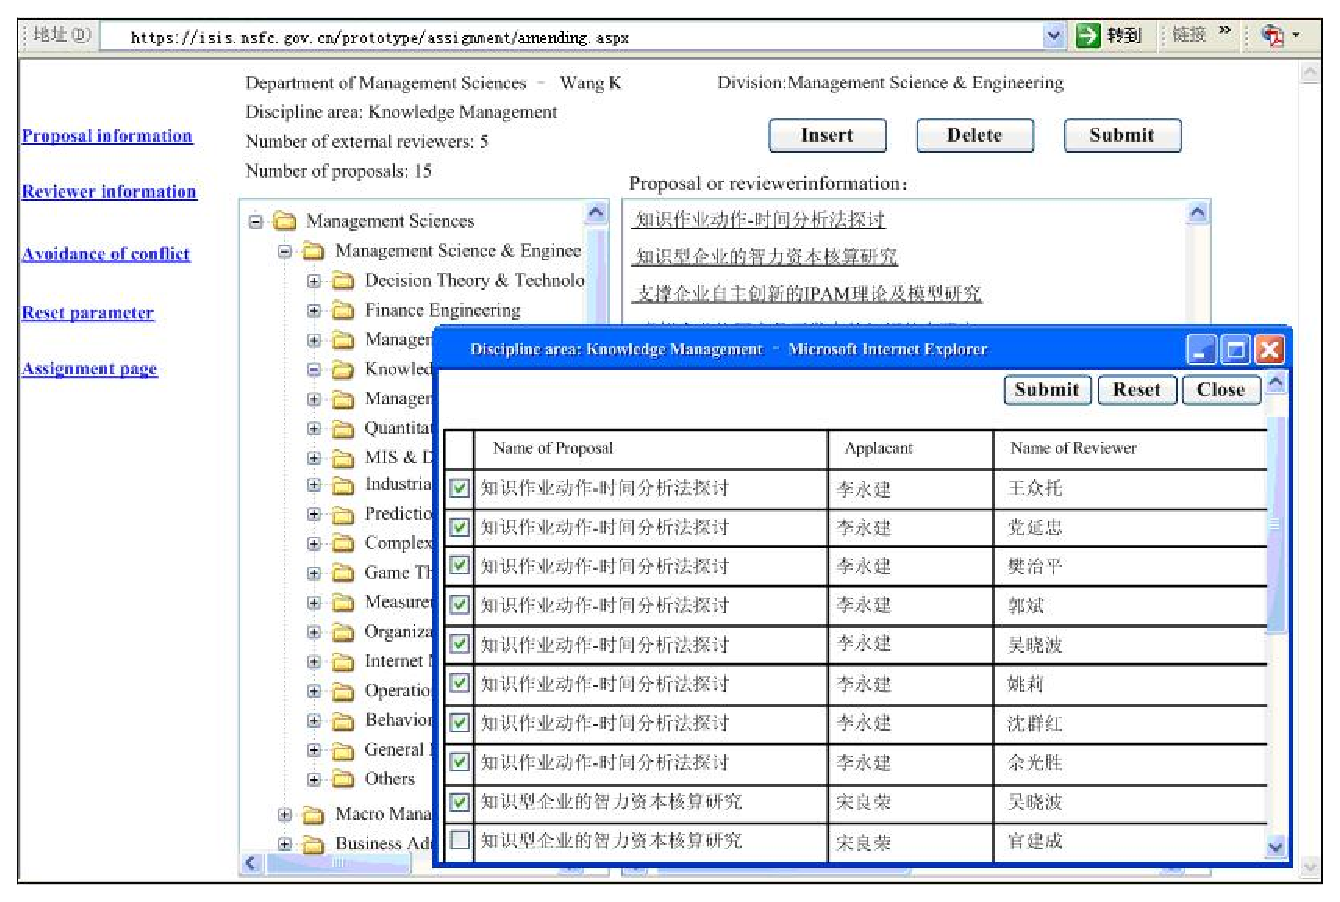
\includegraphics{10}
  \caption{The relationship between the  Clustering Coefficient  and the scale ratio}
\end{figure}

\section{Conclusion and discussion }
\label{sec:5concl-disc-}

In summary, we have proposed a knowledge collaboration network model
based on Wikipedia archive data, and analyze the statistical
properties of the network model. We have found that the
one-dimensional network of this model is a scale-free structure and
its distribution function is subject to the characteristics of the
power law, BA scale-free structure growth and preferential
attachment. From the observation on the changes of the average degree,
the number of the relationships in the knowledge collaboration network
shows cyclical fluctuations, and the links tend to closer. In the
one-dimensional knowledge collaboration network, with the increasing
of network size, the clustering coefficient will be inclined to a
non-zero constant(0.65). Meanwhile, the network average distance is
less than 4, which reflects that the small-world effect exists
obviously in the knowledge collaboration network. 在网络发展初期不具有
明显的等级拓扑结构,随着网络规模的增长,并不显著的表现出等级性。另外,
在知识协同二维网络模型中,话题节点的主题度分布同一维BA一维网络度分布一
样,服从幂律分布,具有“长尾性”等特征。一维网络特性中网络密度随着规模比
的增长而增长,集聚系数则呈现出震荡上升的趋势,有一种不显著的相关性。本
研究还有一些局限性和不足之处,比如数据片段选取的科学性,等级拓扑结构的
阶段性,以及集聚系数与规模比关系等方面尚需进一步讨论。

\section*{Acknowledgment}
\label{sec:acknowledgment}
This work was partly supported by the National Natural Science Foundation of China (NSFC, Project No. 70871006).


\bibliographystyle{elsarticle-num}
\bibliography{../../bibtex/elsevier,../../bibtex/emerald,../../bibtex/chinese,../../bibtex/jstor,../../bibtex/citeseer,../../bibtex/acm,../../bibtex/wiley,../../bibtex/book,../../bibtex/thesis,../../bibtex/ebsco,../../bibtex/old,../../bibtex/ieee,../../bibtex/internet,../../bibtex/ssrn,../../bibtex/apa,../../bibtex/blackwell,../../bibtex/sage,../../bibtex/springer,../../bibtex/MESharp,../../bibtex/taylor}
\end{document}
